\chapter{Meilensteinplanung}
Im Rahmen dieses Projekts war es erforderlich, eine detaillierte Planung und Organisation der Arbeitspakete vorzunehmen.
Um dies zu erreichen, haben wir die Tabelle mit den Arbeitspaketen analysiert und ein Gantt-Diagramm erstellt.
Das Gantt-Diagramm bietet eine visuelle Darstellung der zeitlichen Abfolge und Dauer der verschiedenen Aufgaben, was die Projektplanung und -kontrolle erleichtert.

\section*{Vorgehensweise zur Erstellung des Gantt-Diagramms}
Zunächst haben wir die Daten aus der Tabelle extrahiert und aufbereitet.
Die Tabelle enthielt drei wesentliche Spalten: Arbeitspaket vom, Beschreibung und Dauer.
Diese Daten wurden in ein geeignetes Format gebracht, um sie in das Gantt-Diagramm-Tool einzugeben.
Zur Erstellung des Gantt-Diagramms wurde die Website \texttt{onlinegantt.com} genutzt.
Diese Plattform bietet eine benutzerfreundliche Oberfläche zur Eingabe und Visualisierung von Projektplänen. \newline
Für jedes Arbeitspaket wurde das Startdatum entsprechend der Tabelle eingegeben.
Die Beschreibung der Aufgaben wurde als Titel für die jeweiligen Arbeitspakete verwendet.
Die Dauer der Aufgaben wurde in Tagen oder Wochen entsprechend der Tabelle angegeben.
Nachdem alle Daten eingegeben wurden, generierte die Plattform das Gantt-Diagramm. \newline
Dieses Diagramm ermöglicht es, die zeitliche Abfolge der Aufgaben zu visualisieren und Überschneidungen oder Abhängigkeiten zwischen den Aufgaben zu erkennen.

\section*{Analyse der Zeitplanung}
\subsection*{Gesamtübersicht}
Die Erstellung des Gantt-Diagramms zeigte eine klare Struktur des Projekts, beginnend am 08. März 2024 und endend am 30. April 2024.
Die Aufgaben sind logisch und sequenziell angeordnet, was die Nachverfolgung und Kontrolle erleichtert.

\subsection*{Dauer und Überlappungen}
Einige Aufgaben, wie die Einrichtung des Repositories auf GitHub oder die Erstellung der Projektstruktur, hatten eine kurze Dauer von nur einem Tag.
Andere Aufgaben, wie die Implementierung des Chat-Screens oder die Anpassung der Seiten-Navigation, dauerten mehrere Wochen. \newline
Diese längeren Aufgaben wurden parallel zu kürzeren Aufgaben geplant, um die Gesamtzeit des Projekts effizient zu nutzen.

\subsection*{Wichtige Meilensteine}
Einige wesentliche Meilensteine des Projekts sind:
\begin{itemize}
    \item Die ersten beiden Wochen des Projekts waren der Einrichtung der Entwicklungsumgebungen und der Definition der App-Funktionalitäten gewidmet.
    \item Der Großteil des Projekts, von Mitte März bis Ende April, bestand aus der Implementierung verschiedener Funktionen und der Backend-Integration.
    \item Die letzten Tage des Projekts wurden für Feinanpassungen und Updates, wie die Aktualisierung des Loadingscreens und das Update des Usernames auf dem Accountprofile-Screen, verwendet.
\end{itemize}

\subsection*{Risikobewertung}
Durch das Gantt-Diagramm konnten potenzielle Engpässe und Risiken identifiziert werden. \newline
Aufgaben, die kritische Pfade darstellen, wurden besonders beachtet, um Verzögerungen zu vermeiden.

\begin{figure}[H]
    \caption[Meilensteinplanung]{Meilensteinplanung}
    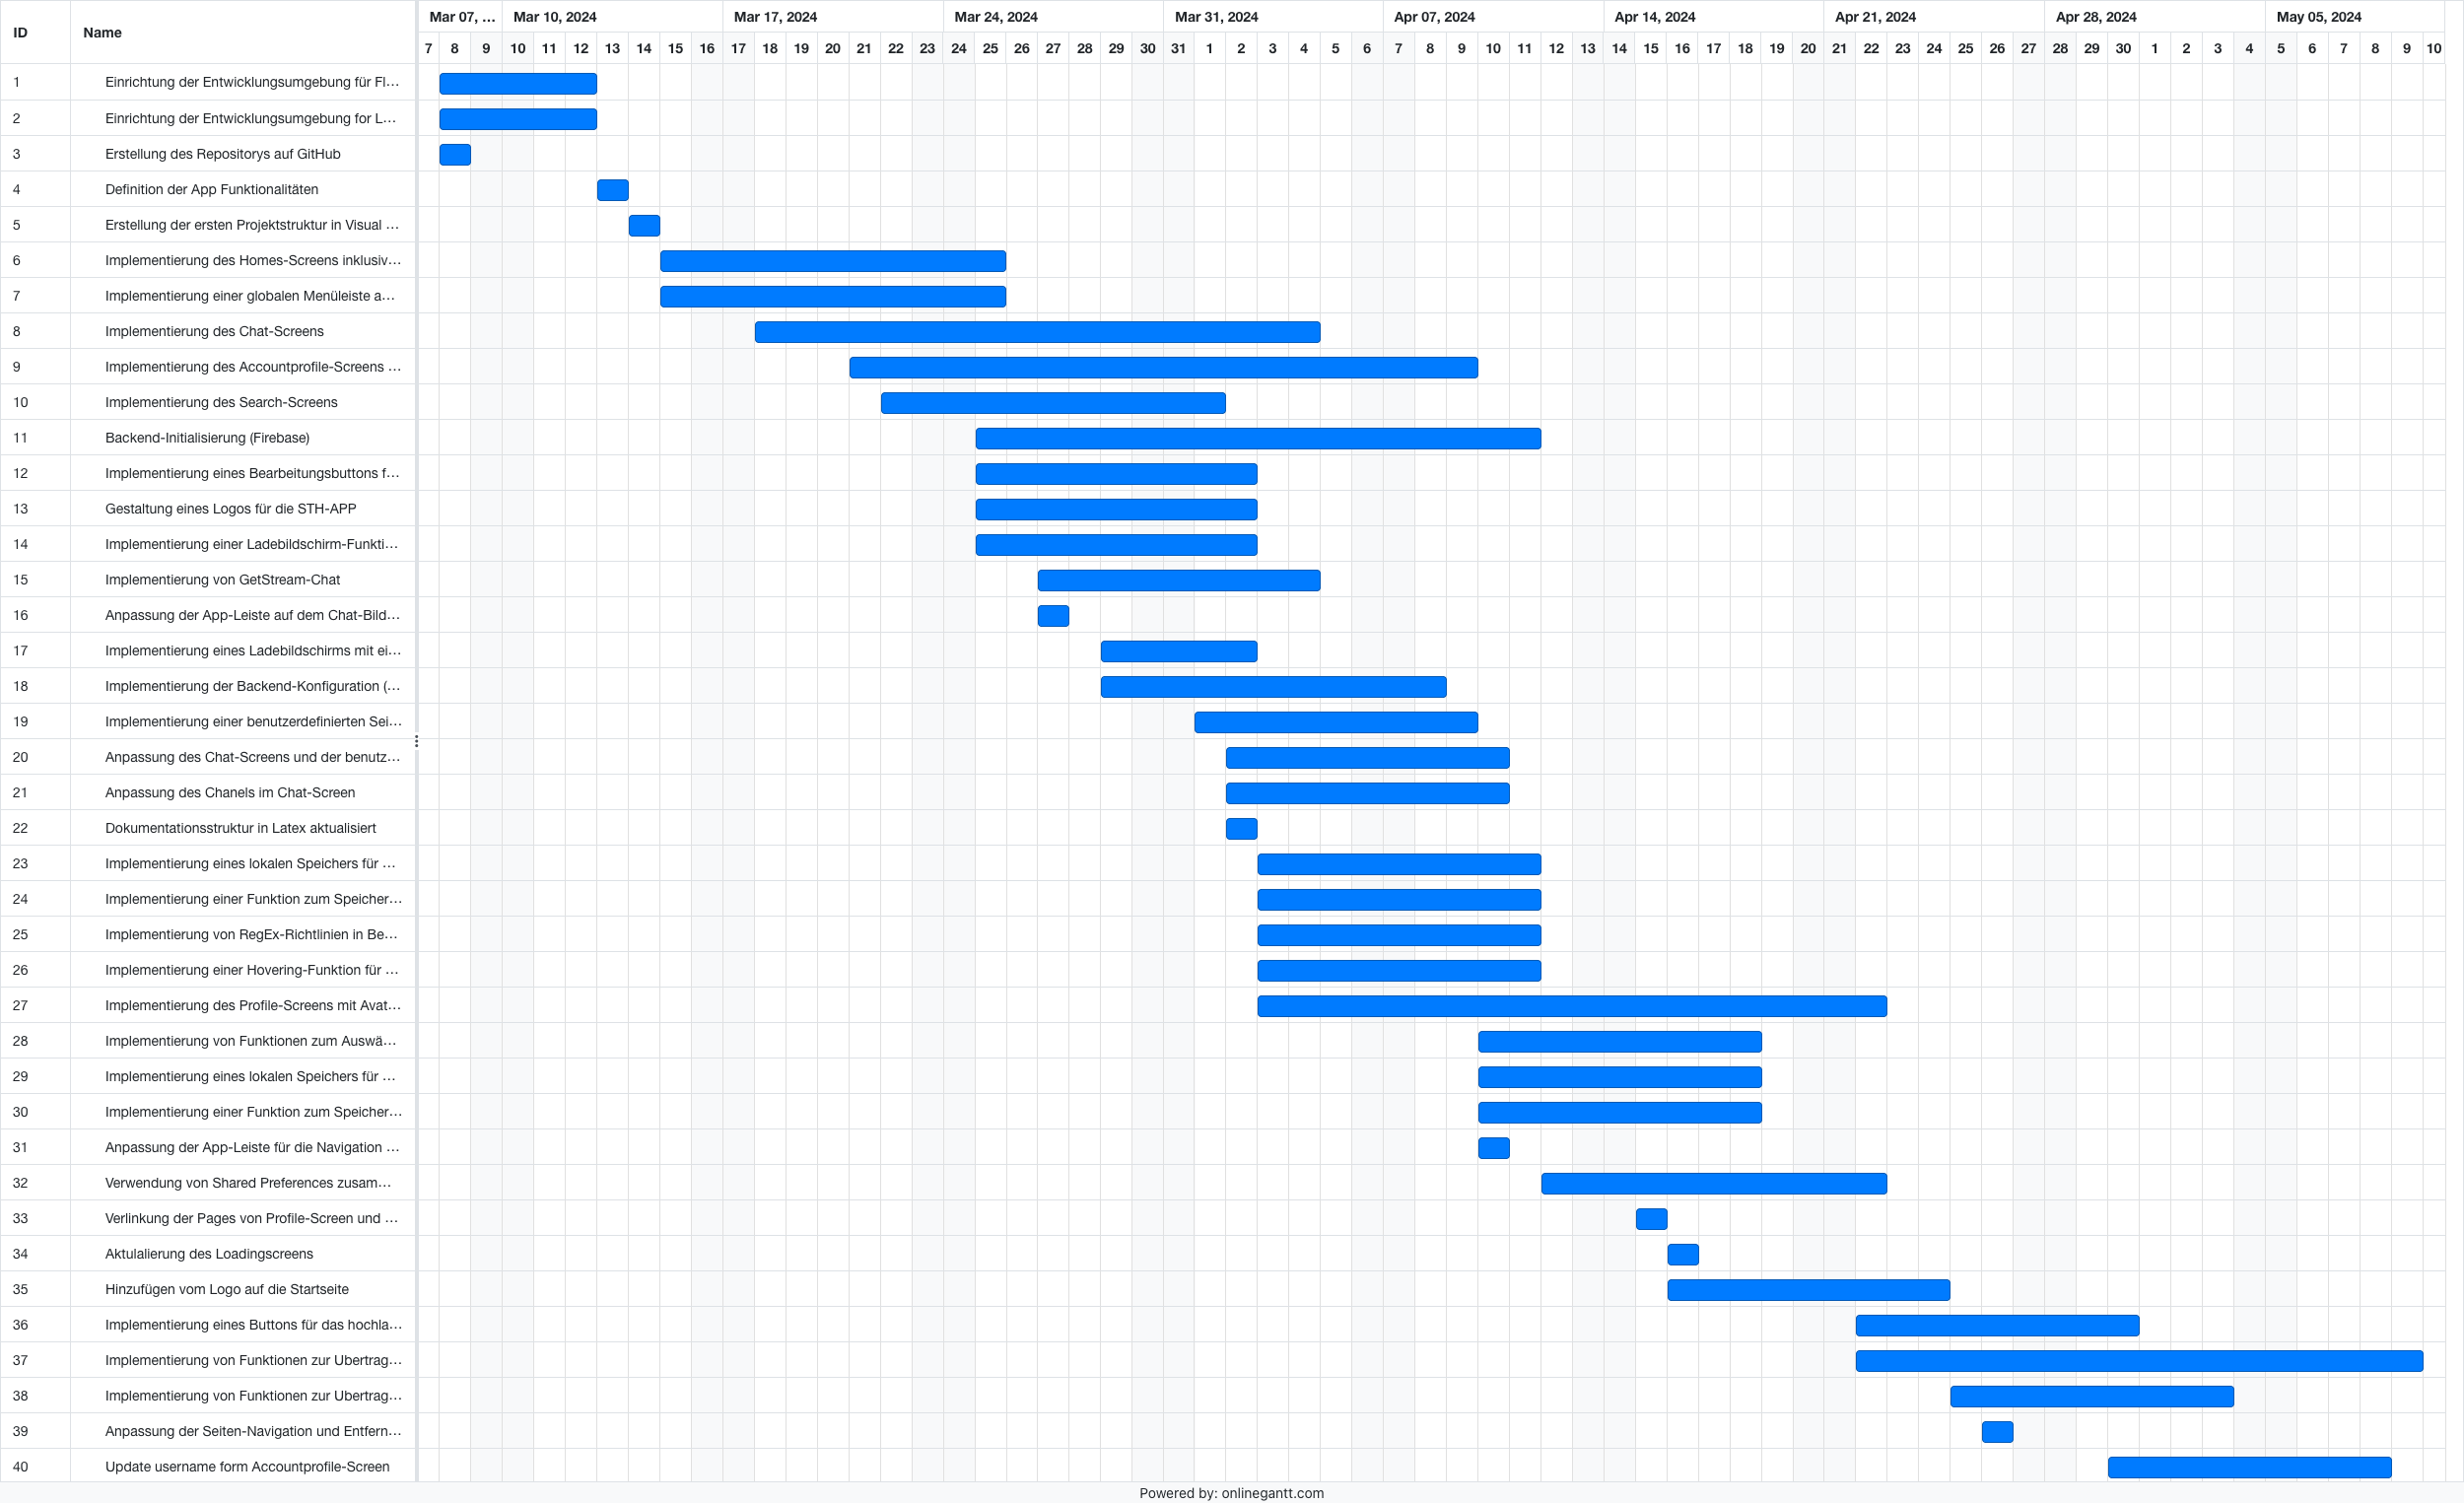
\includegraphics[width=0.9\textwidth]{assets/figures/STH GANTT Diagramm.png}
    \\
    Quelle: \url{https://www.onlinegantt.com}
\end{figure}
